\section{Veruchsaufbau und Durchführung}
\label{sec:Veruchsaufbau}

\begin{figure}[htbp]
    \centering
    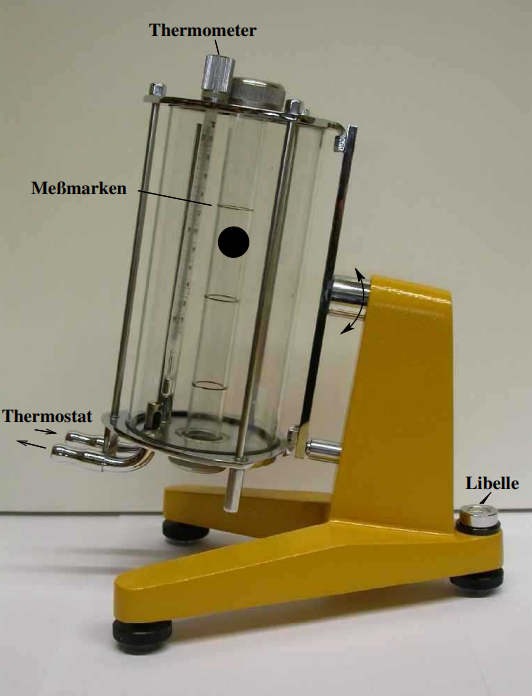
\includegraphics[width=0.7\textwidth]{bilder/hoeppler_viskosimeter.png}
    \caption{Höppler-Viskosimeter}
    \label{fig:hoeppler}
\end{figure}

Für die Versuchsdurchführung wird ein Kugelfall-Viskosimeter nach Höppler benötigt. Das Viskosimeter besteht aus einem Zylinder, in den Wasser eingefüllt ist. 
In diesen ist zentral eine Röhre mit drei Messmarkierungen im Abstand von $5\;\unit{cm}$ eingefasst. 
Das Wasser in dem äußeren Zylinder kann über ein externes Thermostat erhitzt werden. Mit der Libelle und den verstellbaren Füßen lässt sich das Viskosimeter justieren, um
eine eventuelle Schieflage zu korrigieren. In die Röhre wird Wasser eingefüllt. Hierbei ist zu beachten, dass sich keine sichtbaren Luftbläschen bilden. Nun wird die Kugel ebenfalls in die Fallröhre eingefügt und 
der Deckel verschlossen.
Damit keine Wirbel entstehen ist es wichtig, dass das Fallrohr leicht schräg ist, damit die Kugel an der Wand herunterrutscht und nicht anschlägt.

